\documentclass[a4paper,11pt]{report}

\usepackage[T1]{fontenc}
\usepackage[utf8]{inputenc}
\usepackage[italian]{babel}

\usepackage{wrapfig}
\usepackage{mathtools}
\usepackage{graphicx}
\usepackage{amsfonts}
\usepackage{amsthm}
\usepackage{amsmath}
\usepackage{amssymb}
\usepackage{fancyhdr}
\usepackage{float}
\usepackage{geometry}
\geometry{a4paper, top=2.5cm, bottom=2cm, left=2cm, right=2cm}
\usepackage{hyperref}
\hypersetup{
	colorlinks=true,
	linkcolor=black,
	filecolor=blue,
	citecolor = black,      
	urlcolor=cyan,
}

\swapnumbers
\theoremstyle{remark}
\newtheorem*{oss}{Oss}
\newtheorem*{nb}{N.B}
\newtheorem*{coro}{Corollario}
\theoremstyle{definition}
\newtheorem*{teo}{Teorema}
\newtheorem*{Def}{Def}

\newcommand{\C}{\mathbb{C}}
\newcommand{\R}{\mathbb{R}}

\DeclarePairedDelimiter{\abs}{\lvert}{\rvert}

\begin{document}
	\date{}
	\author{Marco Militello}
	\title{Matematica per la fisica}
	\maketitle
	\tableofcontents
	\newpage
	
\part{Analisi complessa}

\chapter{Numeri complessi}
\begin{Def}
	Un numero complesso è una coppia ordinata $(a,b)$ con $a,b \in \R$ tale che siano definite
	\begin{center}
	\begin{tabular}{ll}
		 Addizione  & $[(a,b)+(c,d) = (a+c, b+d)]$\\
		 Moltiplicazione & $[(a,b)(c,d) = (ac-bd, ad+bd)]$ \\
		 Relazione di equivalenza & $[(a,b) = (c,d) \iff a=c \; b=d]$
	\end{tabular}
 	\end{center}
\end{Def}
\begin{teo}
	\[\C = \{(a,b)\, | \, a,b \in \R\}\]
	è un campo Abeliano rispetto addizione e moltiplicazione
\end{teo}
\begin{oss}\hfil
	\begin{itemize}
		\item Proprietà commutativa e associativa seguono da quelle dei reali
		\item Identità additiva \quad $(0) \rightarrow (0,0)$
		\item Esiste opposto: \quad $(a,b) + (-a,-b) = (0,0)$
		\item Identità moltiplicativa: \quad $(1) \rightarrow (1,0)$
		\item Esiste inverso: \quad $(a,b)\frac{1}{(a,b)}= (1,0) \; \frac{1}{(a,b)} = \left(\frac{a}{a^2+b^2}, -\frac{b}{a^2+b^2}\right)$
	\end{itemize}
\end{oss}
\begin{teo}\hfill\\
	Il sottoinsieme $\C_0 = \{(a,0) \, | \, a \in \R\} \subset \C$ è un campo rispetto ad addizione e moltiplicazione \newline
	$\C_0$ è ISOMORFO a $\R$
\end{teo}
\begin{Def}{\textbf{Unità immaginaria}}
	\[(0,1) = i\]
	$(0,1)(0,1) = (-1,0) \qquad (0,-1)=-i$
\end{Def}
\begin{Def}[\textbf{Forma cartesiana}]
	\[z = (a,b) = a + ib \qquad a,b \in \R; \, z \in \C\]
	$a = Re\{z\} \quad b=Im\{z\}$
\end{Def}
\begin{Def}[\textbf{Coniugazione complessa}]
	\[\bar{z} = a-ib = (a,-b) \quad z = a+ib = (a,b)\]
\end{Def}
Operazioni notevoli:
\begin{itemize}
	\item $z + \bar{z} = 2Re\{z\} = 2a$
	\item $z-\bar{z} = 2iIm\{z\} = 2ib$
	\item  $z\bar{z} = a^2+b^2 = \abs{z}^2$
\end{itemize}

\section{Piano complesso (Armand-Gauss)}
\begin{figure}
	\centering
	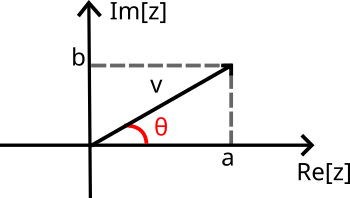
\includegraphics[width=0.4\linewidth]{immagini/piano_gauss}
\end{figure}
\begin{gather*}
	\abs{\vec{v}} = \abs{z} = \sqrt{a^2+b^2} \\
	\begin{cases}
		a = \abs{z}\cos\theta \\
		b = \abs{z}\sin\theta
	\end{cases}
\end{gather*}
Somma come somma vettoriale
\begin{Def}[\textbf{Coordinate polari}]
	\[z = a+ib = r(\cos\theta + i \sin\theta) \quad r= \sqrt{a^+b^2} \quad \tan\theta = \frac{b}{a}\]
	\[\arg(z)=\theta=
	\begin{cases}
		\arctan\left(\frac{b}{a}\right) & a>0 \\
		\arctan\left(\frac{b}{a}\right) + \pi & a<0 \; b>0 \\
		\arctan\left(\frac{b}{a}\right) -\pi & a<0 \; b<0 \\
		\frac{\pi}{2} & a=0 \; b>0 \\
		-\frac{\pi}{2} & a=0 \; b<0
	\end{cases}\]
\end{Def}
\subsection*{Formula di Eulero}
Estendere $e^\gamma \quad \text{con } \gamma \in \R$ \; a \; $e^z \quad \text{con } z \in \C$ 
\[e^z = e^x(\cos(y)+i\sin(y))\]
\begin{oss}
	\begin{gather*}
		z = re^{i\theta} \rightarrow \bar{z} = re^{-i\theta} \\
		z_1z_2 = r_1r_2e^{i(\theta_1 + \theta_2)}
	\end{gather*}
\end{oss}
\subsection*{Formula di De Moivre}
Se $n \in \mathbb{Z} $ si ha:
\[z^n = r^n(\cos(n\theta) +i \sin(n\theta))\]
\subsection*{Radice n-esima}
Se $n \in \mathbb{Z}$ si ha:
\[z^{\frac{1}{n}} = \sqrt[n]{r} \left(\cos\left(\frac{\theta + 2k\pi}{n}\right) + i\sin\left(\frac{\theta + 2k\pi}{n}\right)\right)\]
Allora esistono n diverse radici si $z$ se $\abs{z} \neq 0$
\subsection*{Equazioni di secondo grado in $\C$}
\[az^2+bz+c \qquad \text{con } a,b,c \in \R \; z \in \C\]
Ha sempre 2 soluzioni 
\begin{itemize}
	\item[*] Se $\Delta = b^2 - 4ac \geq 0 \; \Rightarrow$ 2 soluzioni reali
	\item[*] Se $\Delta <0 \; \Rightarrow -\Delta >0 \Rightarrow z_{1,2} \in \C \text{ e } z_1 = \bar{z}_2$
\end{itemize}
\subsection*{Logaritmo}
\[\log(z) = \log(r) + i\phi\]
Così definito il logaritmo è una funzione palindroma, cioè assume valori differenti a seconda $\theta \mapsto \theta + 2k\pi$
Allora scelgo $\theta$ per aver $\log(z)$ univoco
\[\theta \in
\begin{cases}
	[0,\pi] & y>0 \\
	[-\pi,0] & y<0
\end{cases}\]
\begin{nb}
	$\log(z)$ è discontinuo per $x \in (-\infty,0]$ \newline
	Allora escludo $(-\infty,0] \Rightarrow \C \smallsetminus (-\infty,0) \Rightarrow$ BRANCH CUT
\end{nb}
\noindent Definiamo 
\[\log(z) = \log(r) +i\arg(z)\]
$\overline{\log(z)} = \log(\bar{z})$
\subsection*{Norma}
Su $\C$ è definita la norma $\abs{z}$ che soddisfa le proprietà di una distanza $d(a,b) \quad a,b \in \C$
\begin{itemize}
	\item $d(a,b) = d(b,a)$
	\item $d(a,b) = 0 \iff a=b$
	\item $\forall c \in \C \Rightarrow d(a,b) + d(b,c) \geq d(a,c)$
\end{itemize}
\noindent \'E possibile allora definire la distanza 
\[d(z_1,z_2) = \abs{z_1-z_2} \qquad z_1,z_2 \in \C \]
\begin{Def}[\textbf{Successione di Cauchy}]\hfill\\ \label{cauchy}
	\[\{z_k\} \; \text{tale che} \; \forall \epsilon>0 \; \exists N_\epsilon>0 \; | \; \forall n,m>N_\epsilon \Rightarrow \abs{z_n-z_m}<\epsilon\]
\end{Def}
\begin{nb}\hfill
	\begin{enumerate}
		\item $\{z_k\}$ è di \hyperref[cauchy]{Cauchy} se lo sono anche $\{Re(z_k)\} \text{ e } \{Im(z_k)\}$ 
		\item Tutte le successioni convergenti sono di \hyperref[cauchy]{Cauchy}; in $\C$ è vero anche il viceversa perchè $\C$ è completo
	\end{enumerate}
\end{nb}
\begin{Def}[\textbf{Serie su $\C$}]\hfil\\
	La serie $\sum_n z_n$ con $z_n \in \C$ converge a $z \in \C$ se la successione delle somme parziali $\{S_n\}$ converge a $z$
	\[S_n = \sum_{k=0}^{n-1} z_n\]
\end{Def}
\newpage
\begin{oss}\hfil
	\begin{itemize}
		\item Condizione necessaria convergenza: \quad $z_n \to 0 \text{ per } n \to \infty$
		cioè 
		$\begin{cases}
			Re(z_n) \to 0 \\
			Im(z_n) \to 0
		\end{cases}$
		\item Condizione sufficiente: CONVERGENZA ASSOLUTA cioè \newline
		Se converge $\sum \abs{z_n}$  su $\R \Rightarrow$ converge anche $\sum z_n$ su $\C$
	\end{itemize}
\end{oss}
\begin{Def}
	\[e^{i\theta} = \sum_{n=0}^{\infty} \frac{1}{n!} {(i\theta)}^n\]
\end{Def}
\begin{oss}
	$e^{i\theta} = \cos\theta + i\sin\theta$
\end{oss}
\begin{Def}[\textbf{Serie di potenze}]\hfil\\
	$S(z,z_0)$ con $z,z_0 \in \C \text{ e } z_0$ centro si ha:
	\[S(z,z_0) = \sum_{n=0}^{\infty} a_n {(z-z_0)}^n \quad an=cost \, \in \C\]
\end{Def}
\noindent Convergenza per ogni $z$ fissato $\Rightarrow$ 	CONVERGENZA PUNTALE
\begin{oss}
	\[E = \{z \in \C \; | \; S(z,z_0) \text{ è convergente}\}\]
	$E$ non è mai vuoto $\rightarrow z_0 \in E$ e $S(z,z_0) = a_0$ cioè converge 
\end{oss}
\begin{Def}[\textbf{Raggio di convergenza}] \label{def:raggio conv} 
	\[D = \{\abs{z-z_0} \; \forall z \in E\}\]
	Raggio di convergenza:
	\[R = \sup_{z \in E} D\]
	cioè la maggior distanza da $z_0$ per cui la serie converge
\end{Def}
\begin{oss}\hfil
	\begin{itemize}
		\item Le serie di potenze su $\C$ convergono in un cerchio di raggio $R$
		\item Se la serie converge solo in $z=z_0 \Rightarrow R=0$
		\item Se la serie converge $\forall z \in \C \Rightarrow R=\infty$
	\end{itemize}
\end{oss}
\subsubsection*{Calcolo del raggio di convergenza}
\begin{enumerate}
	\item $ \displaystyle R = {\left(\lim_{n \to \infty} \sup_{k \geq n} {\abs{a_k}}^\frac{1}{k}\right) }^{-1}$ \newline
	Si riduce a $\displaystyle \lim_{n \to \infty} \frac{1}{{\abs{a_n}}^{\frac{1}{n}}}$ se tale limite esiste
	\item  $\displaystyle R =\lim_{n \to \infty} \frac{\abs{a_n}}{\abs{a_{n+1}}}$ se tale limite esiste 
\end{enumerate}
\noindent Calcolato $R \Rightarrow$ 
$\begin{cases}
	\abs{z-z_0}<R & \text{la serie converge} \\
	\abs{z-z_0}>R & \text{la serie diverge} \\
	\abs{z-z_0}=R & \text{si studia caso per caso}
\end{cases}$
\begin{oss}
	La derivata di una serie di potenze con raggio di convergenza $R$ ha lo stesso raggio di convergenza
\end{oss}
\begin{coro}
	Una serie di potenze è infinitamente differenziabile all'interno del suo raggio di convergenza
\end{coro}
\chapter{Funzioni complesse}
\begin{Def}[\textbf{Funzione complessa}] \label{def:f complessa} \hfil\\
	Una funzione complessa è una mappa 
	\[f: \, \C \to \C \]
	che associa un punto $z \in \C$ a un punto $w = f(z) \in \C$
	\[f(z) = Re(f(z)) + iIm(f(z)) \Rightarrow f(z) = u(x,y) + iv(x,y)\]
	$u,v$ funzioni su $\R^2$ di $x,y \in \R$
\end{Def}
\begin{Def}[\textbf{Continuità}] \label{def:continuità} \hfill\\
	$f(z)$ è continua in $z_0 \in \C$ se è definita in un intorno di $z_0$ ed esiste finito il limite 
	\[\lim_{z \to z_0} f(z) = f(z_0)\]
\end{Def}
\begin{Def}[\textbf{Limite}]\label{def:limite}\hfil\\
	$f(z_0)$ è il limite di $f(z)$ per $z \to z_0$ se:
	\[\forall \epsilon>0 \; \exists \delta>0 \; | \; \abs{z-z_0}<\delta \text{ se } \abs{f(z)-f(z_0)}<\epsilon\]
\end{Def}
\begin{nb}
	Come per $\R^2$ il limite deve essere indipendente dal cammino
\end{nb}
\begin{Def}[\textbf{Continuità su un dominio}]\hfil\\
	$f(z)$ è continua su un $D \subseteq \C$ se è continua $\forall z \in D$
\end{Def}
\begin{Def}[\textbf{Derivata si una funzione continua}]\hfil\\
	$f(z)$ è differenziabile se esiste il limite
	\[\lim_{z \to z_0} \frac{f(z)-f(z_0)}{z-z_0} = f'(z_0) = \frac{df}{dz}\Bigr|_{z_0}\]
\end{Def}
\begin{nb}
	Anche la derivata è indipendente dal cammino
\end{nb}
\begin{Def}[\textbf{Funzione olomorfa}]\label{def:olomorfa}\hfil\\
	Una funzione differenziabile su $D \subseteq \C$ si dice OLOMORFA
\end{Def}
\subsubsection*{Proprietà funzioni olomorfe}
\begin{itemize}
	\item $(f \pm g)' (z) = f'(z) \pm g'(z)$
	\item $(fg)'(z) = f'(z)g(z) + f(z)g'(z)$
	\item $\left(\frac{f}{g}\right)'(z) = \frac{f'(z)g(z) - f(z)g'(z)}{g^2(z)} \quad g(z) \ne 0$ 
	\item Funzione composta: \quad $\frac{d}{dz} (f \circ g) (z) = f'(g(z))g'(z)$
	\item Derivata funzione inversa: data $w= f(z)$ olomorfa in $z_0$ con $f'(z_0)$ \newline
	$h(w) = z = f^{-1}(w) \text{ è olomorfa in } w_0=f(z_0) \text{ e } h'(w_0) = \frac{1}{f'(h(w_0))} = \frac{1}{f'(z_0)}$
\end{itemize}
\section{Condizioni di Cauchy-Riemann}
Condizioni necessarie e sufficienti per verificare differenziabilità
\begin{teo}\hfill\\
	$f(z) = u(x,y) + iv(x,y)$ tale che $u,v$ abbiano derivate parziali continue in un intorno di $z_0 = x_0 + iy_0$
	 \[\delta_x f(z_0) = i\delta_y f(z)\] cioè:
		\begin{itemize}
			\item $\delta_x u(x,y) \bigr|_{(x_0,y_0)} = \delta_y v(x,y) \bigr|_{x_0,y_0}$
			\item $\delta_y u(x,y) \bigr|_{(x_0,y_0)} = -\delta_x v(x,y) \bigr|_{x_0,y_0}$
		\end{itemize}
\end{teo}
\begin{oss}
	Le condizioni di Cauchy-Riemann permettono di scrivere le derivate complesse di $f(z) = u +iv$ in 4 modi equivalenti:
	\[f'(z) = \begin{cases}
		\delta_x u + i \delta_x v \\
		\delta_x u - i \delta_y v \\
		\delta_x u - i \delta_y u \\
		\delta_y u + i \delta_x u 
	\end{cases}\]
\end{oss}
\begin{Def}[\textbf{Operatori differenziali in $\bf {z,\bar{z}}$}]
	\begin{gather*}
		\delta_z = \frac{1}{2}(\delta_x - i\delta_y) \\
		\delta_{\bar{z}} = \frac{1}{2}(\delta_x + i\delta_y)
	\end{gather*}
\end{Def}
\begin{teo}\hfil\\
	Se $f(z)$ è olomorfa su un dominio $D \subseteq \C \Rightarrow \delta_{\bar{z}} f(z) =0$
\end{teo}
\begin{Def}[\textbf{Funzioni anti-olomorfe}]\hfil\\
	Una funzione si dice anti-olomorfa se
	\[\frac{\delta}{\delta z} f(z) =0\]
\end{Def}
\begin{oss}
	Si può dimostrare che se $f(z)$ è antiolomorfa $\Rightarrow \bar{f}(z)$ è olomorfa 
\end{oss}
\begin{Def}[\textbf{Funzioni trigonometriche}]
	\[\cos{z} = \frac{1}{2} (e^{iz} + e^{-iz}) \qquad \sin{z} = \frac{1}{2i} (e^{iz} - e^{-iz}) \]
\end{Def}
\begin{Def}[\textbf{Funzioni iperboliche}]
	\[\cosh{z} = \frac{1}{2} (e^z+e^{-z}) \qquad \sinh{z} = \frac{1}{2} (e^z-e^{-z})\]
\end{Def}
\section{Proiezione stereografica e punto all'infinito}
I numeri complessi sul piano $\C$ possono essere rappresentati come punti sulla superficie di una sfera
\[S^2 = \left\{(\xi,\eta,\zeta) \; \Bigr| \; \xi^2 + \eta^2 + {\left(\zeta - \frac{1}{2}\right)}^2 = \frac{1}{4}\right\}\]
\begin{figure}[H]
	\centering
	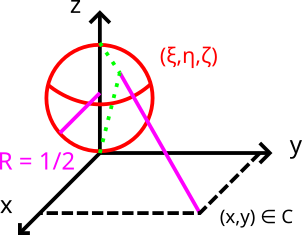
\includegraphics[width=0.6\linewidth]{immagini/sfera}
	\label{fig:sfera}
\end{figure}
\begin{gather*}
	x = \frac{\xi}{1-\zeta} \qquad y = \frac{\eta}{1-\zeta} \\
	\xi = \frac{x}{x^2+y^2+1} \qquad \eta = \frac{y}{x^2+y^2+1} \qquad \zeta = \frac{x^2+y^2}{x^2+y^2+1}
\end{gather*}
\noindent $\zeta =1 \Rightarrow x=y=\infty  \rightarrow (0,0,1)$ è chiamato PUNTO ALL'INFINITO 
\[\C \cup \{\infty\} = S^2 = \hat{\C} \rightarrow \text{ COMPATTIFICAZIONE di } \C\]
$\hat{\C}$ è isomorfo a una sfera
\begin{nb}
	Avremmo potuto usare la proiezione del polo sud $(0,0,-1)$; in questo caso il punto $z=\infty$ sarebbe stato mappato su $w = \frac{1}{x+iy}=0$ \newline
	Quindi per studiare $f(z)$ definita su $\C$ e capire il suo andamento a $z=\infty$ posso studiare $f\left(\frac{1}{w}\right)$ attorno a $w=\infty$ con $w=\frac{1}{z}$ \newline
	Se $f\left(\frac{1}{w}\right)$ è olomorfa o singolare in $w=0 \Rightarrow f(z)$ è olomorfa o singolare in $z=\infty$ 
\end{nb}
\begin{Def}[\textbf{Intera}]\hfil\\
	Se $f(z)$ è olomorfa su tutto $\C \Rightarrow$ si dice INTERA	 
\end{Def}
\begin{Def}[\textbf{Singolarità}]\hfil\\
	I punti in cui $f(z)$ (non intera) non è differenziabile o non è definita si dicono SINGOLARIT\'A
\end{Def}
\section{Singolarità}
\section*{Singolarità isolate}
Se $f(z)$ è olomorfa in un intono di $D(z_0,\epsilon) =\{z \; | \; \abs{z-z_0}<\epsilon\}$ di $z_0$ ma non in $z_0$; se $f(z_0)$ non è definta o non  differenziabile
\begin{enumerate}
	\item \textbf{Singolarità rimovibile} \newline
	Se $f(z_0)$ non è definta, ma esiste finito 
	\[\lim_{z\to z_0} f(z)\]
	posso estendere $f$ in $z_0$ 
	\[f(z_0) = \lim_{z\to z_0} f(z)\] 
	Con questa estensione $f(z)$ estesa è olomorfa in $D \cup \{z_0\}$
	\item \textbf{Singolarità di tipo polo di ordine k} \newline
	Se esiste finito
	\[\lim_{z\to z_0} {(z-z_0)}^kf(z) = a \ne 0 \quad k \in \mathbb{N}\geq 1\]
	allora $f(z)$ ha un polo di ordine k
	\begin{itemize}
		\item K=1 $\rightarrow$ Polo semplice
		\item k=2 $\rightarrow$ Polo doppio
	\end{itemize}
	\begin{oss}
		Nelle vicinanze di un polo di ordine k si può scrivere 
		\[f(z) = \frac{g(z)}{{(z-z_0)}^k} \quad g(z) \text{ olomorfa e non nulla in } z_0\]
	\end{oss}
	\begin{oss}
		dato un polo di ordine k
		\[\lim_{z\to z_0} {(z-z_0)}^kf(z) = \infty \quad \forall k < n\]
		In particolare per $k=0$
		\[\lim_{z\to z_0} f(z)=0 \text{ la funzione diverge ad un polo}\]
	\end{oss}
	\item \textbf{Singolarità essenziale} \newline
	Singolarità non rimovibile neanche moltiplicando per ${(z-z_0)}^n$ con $n\to \infty$ \newline
	Se $f(z_0)$ è singolarità essenziale di $f(z)$ allora non esiste $\lim_{z\to z_0}$ \newline
	$f(z)$ oscilla violentemente tanto più mi avvicino a $z_0$ a seconda del cammino; $f(z)$ può assumere qualsiasi valore
\end{enumerate}
\begin{teo}[\textbf{Weierstrass}]\hfil\\
	$f(z_0)$ singolarità essenziale; posso avvicinarmi quanto voglio alla singolarità essenziale e allo stesso tempo avvicinarmi a qualsiasi complesso
	\[\forall \epsilon,\delta>0 \; \forall c \in \C \Rightarrow \exists z \; | \; \abs{z-z_0}<\delta \text{ e } \abs{f(z)-c}<\epsilon\]
\end{teo}
\begin{teo}[\textbf{Picard}]\hfil\\
	In un intono di $z_0$ singolarità essenziale di $f(z)$ , $f(z)$ assume qualsiasi valore complesso un numero infinito di volte con eccezione al più di un valore
\end{teo}
\begin{Def}[\textbf{Funzione meromorfa}]\hfil\\
	$f(z)$ è MEROMORFA se le sue uniche singolarità in un dominio $D \subseteq \C$ sono rimovibili o poli (non si considerano le singolarità a $z=\infty$)
\end{Def}
	\begin{oss}
		Si possono studiare le proprietà di singolarità di $f(z)$ in z=$\infty$ studiando le proprietà di $f(w)$ con $w=\frac{1}{z}$ in $w=0$ \newline
		Grazie al doppio mapping della proiezione stereografica si ha: 
	\end{oss}
	\begin{itemize}
		\item poli in z $\rightarrow$ zeri in w 
		\item zeri in z $\rightarrow$ poli in w
		\item singolarità essenziali in z $\rightarrow$ singolarità essenziali in w
	\end{itemize} 
	\section*{Singolarità non isolata}
	Singolarità si dice non isolata se non esiste intorno in cui è isolate
	\begin{nb}
		Basta un solo punto $z_1$ tale che $\abs{z-z_0}<\delta$ con $f(z_1)$ non olomorfa per avere che $f(z_0)$ è singolarità non isolata
	\end{nb}
	\begin{enumerate}
		\item Singolarità che sono punti limite di una sequenza di singolarità isolate \newline
		es.: $f(z) = \tan(\frac{1}{z})$
		\item Punti di diramazione di funzioni a più variabili \newline
		es.: $f(z) = \sqrt{z}$
	\end{enumerate}
\chapter{Superfici di Rieamann}
	Una volta fissata la disposizione del branch cut, tutti i valori della funzione in tutti i rami sono fissati sapendo il valore in un punto. \newline
	$f(z)=\sqrt{z}$ definisco cut $(-\infty,0]$ e dico che $\sqrt{1}:=1$; Ho completamente determinato $f(z)$ sia $w_0(z)$ che $w_1(z)$. \newline
	Questo suggerisce che esiste descrizione alternativa in cui non ci sono tagli. \newline
	La funzione a valori doppi sono quindi single-value ed olomorfe. \newline
	Estendo il dominio con molteplici copie di $D \subseteq \mathbb{C}$. \newline
	es.: lo stesso punto $z \in \mathbb{C}$ possiamo immaginare abbia 2 immagini diverse $f(z)$ : $f_1(z)$ e $f_2(z)$ \newline
	Raddoppiando $\mathbb{C}$ avremmo 2 copie $z_1$ e $z_2$ $\Rightarrow$ abbiamo $f_1(z_1)$ e $f_2(z_2)$ che ora sono single-valued. \newline
	Il nuovo dominio si chiama {\bfseries SUPERIFICIE DI RIEMANN}  e corrisponde ad un'estensione di $\mathbb{C}$
	\begin{figure}[h]
		\centering
		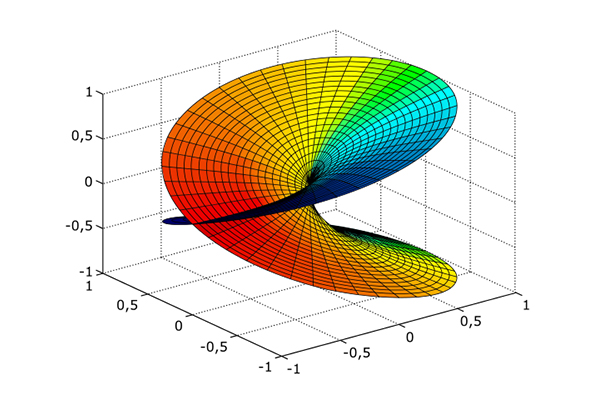
\includegraphics[width=0.7\linewidth]{immagini/riemann.jpg}
		\caption{Superficie di Riemann}
		\label{fig:riemann}
	\end{figure}
	\noindent Le due copie di $\C$ vanno incollate lungo quello che prima era il branch cut. In questo modo attraversando le linee di congiungimento si passa da un ramo all'altro. \newline
	In generale ci sono tante copie di $D \in \mathbb{C}$ quante sono le branch-cut (eventualmente anche infinite [es:~$\log(z)]$)
	\chapter{Integrazione sul piano complesso}	
	Le proprietà di olomorfia di $f(z)$ su $\mathbb{C}$ possono essere determinate dalle condizioni di Riemann. \newline
	Le proprietà di differenziabilità sono connesse con le proprietà di integrabiltà di $f(z) \mbox{ su } \mathbb{C}$ 
	\section{Curve}
	\begin{Def}[\textbf{Curva}] \hfil\\
		Una curva è una mappa continua 
			\begin{gather*}
				\gamma:[a,b] \in \mathbb{R} \rightarrow \mathbb{C} \\
				t \mapsto \gamma(t)= x(t) +iy(t)
			\end{gather*}	
		$z_a = \gamma(a) \mbox{ e } z_b=\gamma(b)$ sono gli estremi della curva 
	\end{Def}
	\begin{Def}[\textbf{Orientazione curva}] \hfil
		\begin{itemize}
			\item Una curva si dice che ha ORIENTAZIONE POSITIVA se il verso di percorrenza è antiorario
			\item Una curva si dice che ha ORIENTAZIONE NEGATIVA se il verso di percorrenza è orario
		\end{itemize}
	\end{Def}
	\begin{Def}[\textbf{Curva opposta}]\hfil\\
		La curva con orientazione opposta è data da una mappa 
		\[t \mapsto \gamma(a+b-t)=-\gamma\]
	\end{Def}
	\begin{Def}[\textbf{Curva semplice}]\hfil\\
		Una curva semplice è una curva che non si interseca $\Rightarrow$ mapping iniettivo
		\[\gamma(t_1)\neq\gamma(t_2) \quad \forall t_1\neq t_2\]
	\end{Def}
	\begin{Def}[\textbf{Curva chiusa}]\hfil\\
		Una curva chiusa è una curva tale che $\gamma(a)=\gamma(b)$ 
	\end{Def}
		\begin{Def}{\textbf{Curva di Jordan}}\hfil\\
		Una curva di Jordan è una curva semplice e chiusa (nessun altro punto oltre a $z_a=z_b$ coincide)
	\end{Def}
	\begin{Def}{\textbf{Curva regolare a tratti}}\hfill\\
		Data una curva $\gamma(t)=x(t)+iy(t)$, se $x(t) \mbox{ e } y(t)$ sono continue per $t\in[a,b]$ e se esiste una partizione di $[a,b]$ dove $x'(t) \mbox{ e } y'(t)$ sono continue e non simultaneamente nulle $\Rightarrow$ $\gamma(t)$ è regolare a tratti.
	\end{Def} 
	\begin{Def}{\textbf{Curve omotope}}\hfil\\
		Due curve su $D \in \mathbb{C}$ con gli stessi estremi $[a,b]$ sono omotope se: esiste una mappa continua che manda l'una nell'altra
		\begin{gather*}
			\gamma:[a,b]\times[0,1] \mapsto D \in \mathbb{C} \mbox{ t.c. se } t=[a,b] \mbox{ e } u=[0,1]: \\
			\forall t \in [a,b] \mbox{ } \forall u \in [0,1] \Rightarrow \gamma(t,0) = 	\gamma_1(t) \mbox{ e } \gamma(t,1)= \gamma_2(t)
		\end{gather*}
		Quindi $\gamma(a,u)=\gamma_1(a)=\gamma_2(a) \mbox{ e } \gamma(b,u)=\gamma_1(b)=\gamma_2(b)$ \newline
		Per ogni valore di u ho una curva in D; variando u passo da $\gamma_1$ a $\gamma_2$ 
	\end{Def} 
		\begin{teo}[\textbf{Jordan}]\hfil\\
			Ogni curva di Jordan divide il piano complesso in 2 regioni. \newline
			Se l'orientazione della curva è positiva a destra ho la regione esterna, mentre a destra ho la regione interna; se l'orientazione è negativa ho l'opposto. 
		\end{teo}
		\begin{Def}{\textbf{Dominio semplicemente connesso}}\hfil\\
			Date due curve $\gamma_1$ e $\gamma_2$ che sono omotope 
			\begin{equation*}
					\forall u \in [0,1] \Rightarrow \gamma(a,u)=\gamma(b,u) \mbox{ e } \gamma(t,0)=\gamma_1(t) 	\mbox{ } \gamma(t,1)=\gamma_2(t)
			\end{equation*}
			Allora il dominio D è semplicemente connesso se ogni curva chiusa è omotopa ad un punto (cioè può essere deformata in punto). \newline
			Ciò è possibile solo se non ci sono buchi.
		\end{Def}
	\section{Integrale di linea}
	\begin{Def}[\textbf{Integrale di linea}]\hfil\\
		Data una curva regolare a tratti $\gamma: t\mapsto\gamma(t)=x(t)+iy(t) \text{ con } t \in [a,b]\subseteq\mathbb{C}$ \newline
		Dato un dominio $D\subseteq\mathbb{C}$ e una funzione $f(z) \mbox{ con } z=\gamma(t)$ che sia continua $\forall z=\gamma(t)\in D \mbox{ e } \forall t \in [a,b]$ $\Rightarrow$ si definisce INTEGRALE DI LINEA di f lungo $\gamma$
		\begin{equation*}
		\int_\gamma f(z)\,dz = \int_{a}^{b} f(\gamma(t))\gamma'(t)\,dt \quad \mbox{ con }\gamma'(t) = \frac{d\gamma(t)}{dt} = x'(t)+iy'(t)
		\end{equation*}
		Si ha dunque 
		\begin{equation*}
			\int_\gamma f(z)\,dz = \int_{a}^{b} \bigl[u(x(t),y(t)) + iy(x(t),y(t))\bigr]\bigl(x'(t)+iy'(t)\bigr)\,dt \quad \text{con } f(z)= u(x,y)+iv(x,y)
		\end{equation*}
		\begin{equation*}
		\int_\gamma f(z)\,dz = \int_{a}^{b} (ux'-vy')\,dt + i\int_{a}^{b} (uy'+vx')\,dt
		\end{equation*}
	\end{Def}
	\begin{oss}
		Questo ci dice l'integrale è lineare e i cammini possono essere sommati
		\begin{gather*}
			\int_\gamma af(z)+bf(z)\,dz = a\int_\gamma f(z)\,dz + b\int_\gamma f(z)\,dz \quad \forall a,b \in \mathbb{C} \\
			\int_{\gamma_1} f(z)\,dz + \int_{\gamma_2} f(z)\,dz = \int_{\gamma_1+\gamma_2} f(z)\,dz \quad \mbox{se } \gamma_1(b)=\gamma_2(a)
		\end{gather*}
		Questa proprietà mi permette di scrivere $	\int_\gamma f(z)\,dz= -\int_{-\gamma} f(z)\,dz$
	\end{oss}
	\begin{oss}
		L'integrale è indipendente dalla parametrizzazione scelta per la curva $\gamma$
	\end{oss}
	\begin{Def}[\textbf{Lunghezza curva}]
		\begin{equation*}
			L=\int_{a}^{b} \abs{\gamma'(t)}\,dt = \int_{a}^{b} \sqrt{(x'(t))^2+(y'(t))^2}\,dt
		\end{equation*}
	\end{Def} 
	\begin{teo}[\textbf{Disuguaglianza di Darboux}]\hfil\\
		Data una curva regolare a tratti $\gamma(t)$ di lunghezza L e una funzione $f(z)$ continua e limitata su $\gamma$
		\begin{equation}
			\abs{f(z)}\le M \quad \forall z \in \gamma \Rightarrow \abs*{\int_\gamma f(z)\,dz}\le LM
		\end{equation}
	\end{teo}

\section{Valore principale integrale}
	Generalizzo il concetto di integrale improprio \newline
	se $f(z)$ è continua su una curva $\gamma(t)$ con $t\in [a,b]$ ad eccezione di un punto $\xi \in \gamma(t)$ \newline
	Posso considerare una circonferenza di raggio $\epsilon$ intorno a $\xi$ \newline
	Definisco 
	\begin{equation*}
		I_a = \int_{a}^{\xi'} f(\gamma(t))\gamma'(t)\,dt \text{ e } I_b = \int_{\xi''}^{b} f(\gamma(t))\gamma'(t)\,dt \quad \forall \epsilon>0	
	\end{equation*}
	Se esistono $I_a, I_b \mbox{ per } \epsilon\to 0 \Rightarrow I_a + I_b$ è integrale improprio di $f(z)$ lungo $\gamma$ \newline
	Se $I_a \mbox{ o } I_b \to\pm\infty \mbox{ quando } \epsilon \to 0 \mbox{ ma } \displaystyle \lim_{\epsilon\to 0} I_a + I_b = a (finito) \in \mathbb{C}
	\Rightarrow$ si definisce il valore principale 
	\begin{equation*}
		P.V. \int_\gamma f(z)\,dz = \lim_{\epsilon \to 0} \Bigl(\int_{a}^{\xi'(t)} f(z)\,dz + \int_{\xi''(t)}^{b} f(z)\,dz\Bigr)
	\end{equation*}

	\begin{nb}
		Se le singolarità sono più di una si può scrivere
		\begin{equation*}
			P.V. \int_\gamma f(z)\,dz =\lim_{\epsilon \to 0} \Bigl(\sum_{j=0}^{n} \int_{\xi''_j}^{\xi''_{j+1}} f(z)\,dz\Bigr) \quad \text{con } \xi''_0=a \quad \xi'_{n+1}=b
		\end{equation*} 
	\end{nb}
 
\chapter{Forme differenziali}
	\begin{Def}[\textbf{Forma differenziale}]\hfil\\
		$\omega = P(x,y)dx + Q(x,y)dy \quad$ con P,Q funzioni $C^1 \mbox{ su } D \subseteq \mathbb{R}^2$
	\end{Def}

	\begin{Def}[\textbf{Integrale di una forma differenziale}]\hfil\\
		L'integrale di una forma differenziale su una curva $\gamma(t)$ regolare a tratti è:
		\begin{equation*}
			\int_\gamma \omega = \int_{a}^{b} \bigl[P(x(t),y(t))x'(t)+Q(x(t),y(t))y'(t)\bigr]\,dt \Rightarrow \int_\gamma \omega = \int_\gamma f(z)
		\end{equation*} 
	\end{Def}
	
	\begin{teo}[\textbf{Green}]\hfil\\
		Data una forma differenziale definita su S racchiuso da una curva di Jordan $\gamma$ con orientazione positiva 
		\begin{equation}
			\int_\gamma P(x,y)dx + Q(x,y)dy\,dt = \iint_S \bigl[\delta_x Q(x,y)- \delta_y P(x,y)\bigr]\,dx\,dy
		\end{equation}
	\end{teo}

	\begin{teo}[\textbf{Cauchy}]\hfil\\
		Sia $f(z)$ olomorfa su D semplicemente connesso e $\gamma$ una curva chiusa in D 
		\begin{equation*}
			\int_\gamma f(z)\,dz = 0
		\end{equation*}
	\end{teo}

	\begin{oss}
		Esiste un'estensione dovuta a Goursat che non richiede che $f(z)$ sia derivabile su un dominio semplicemente connesso, ma basta chiedere che $f(z)$ sia omotopa ad un punto.
	\end{oss}

	\begin{coro}
		L'integrale di una funzione $f(z)$ olomorfa su D semplicemente connesso non dipende dal cammino $\gamma$
	\end{coro}

	\begin{oss}
		In generale se D non è semplicemente connesso il teorema fallisce.
	\end{oss}
	\begin{teo}\hfil\\
		Sia $f(z)$ olomorfa su un dominio D. Per un punto arbitrario $z_0 \in D $ possiamo sempre definire la primitiva 
		\begin{equation*}
			F(z)=\int_{z_0}^{z} f(z')dz
		\end{equation*}
		$F(z)$ è anch'essa olomorfa e si ha che $F'(z)= f(z)$
	\end{teo}

	\begin{coro}\hfil
		\begin{enumerate}
			\item Due diverse primitive di $f(z)$ possono differire solo per una costante.
			\item $\int_{A}^{B} f(z)\,dz = F(B)-F(A)$
		\end{enumerate}
	\end{coro}

\section{Relazione tra forme differenziali e campi vettoriali}
	Usando le condizioni di Cauchy-Riemann la forma differenziale su può scrivere come:
	\[\omega = f(z)dz = (u+iv)dx + (-v+iu)dy\]

	\begin{Def}[\textbf{Forma differenziale chiusa}]\hfil\\
		$\omega = P(x,y)dx + Q(x,y)dy$ \quad si dice chiusa se $\delta_y P = \delta_x Q$
	\end{Def}

	\begin{Def}[\textbf{Forma differenziale esatta}]\hfil\\
		$\omega = dg = \delta_x g(x,y)dx + \delta_y g(x,y)dy$
	\end{Def}

	\begin{oss}
		Ogni forma differenziale esatta è anche chiusa: $\delta_x\delta_y g(x,y) = \delta_y\delta_x g(x,y)$
	\end{oss}
\section{Formula integrale di Cauchy}

	\begin{teo}\hfil\\
		Data $f(z)$ olomorfa su D semplicemente connesso e data $\gamma$ di Jordan con orientazione positiva 
		\[\Rightarrow \forall z_0 \mbox{ interno a } \gamma \text{ si ha: } \quad 
		f(z_0) = \int_\gamma \frac {f(z_0)}{z-z_0} \,dz\]
	\end{teo}

	\begin{oss}
		Questo permette di costruire il valore di $f(z)$ all'interno di $\gamma$ partendo dai valori di $\gamma$ che sono il bordo della regione $\Rightarrow$ OLOGRAFIA
	\end{oss}

	\begin{coro}
		Se $f(z)$ è olomorfa in $z_0$ $\Rightarrow$ è differenziabile infinite volte e ha derivate che si possono scrivere come: 
		\[f^{(n)}(z_0)= \frac{n!}{2\pi i} \int_\gamma \frac{f(z)}{(z-z_0)^{n+1}} \, dz\]
		La formula integrale di Cauchy è un caso particolare per curve semplici e chiuse. Se la curva non è semplice si può avvolgere più volte attorno a $z_0$
	\end{coro}

	\begin{Def}[\textbf{Numero avvolgimenti}]
		\[n(\gamma,z_0) = \frac{1}{2 \pi i} \int_\gamma \frac{1}{z-z_0}\,dz \quad
		\Rightarrow \quad n(\gamma,z_0)f(z_0) = \frac{1}{2 \pi i} \int_\gamma \frac{f(z)}{z-z_0}\,dz\]
	\end{Def}

	\begin{teo}\hfil\\
		Data $\gamma(t)$ con $t \in [a,b]$ curva chiusa e dato $z_0 \notin \gamma$ si ha che $n(\gamma,z_0) \in \mathbb{Z}$
	\end{teo}

	\begin{Def}[\textbf{Funzione analitica}]\hfil\\
		Se $F(z)$ è olomorfa su un cerchio $D_R$ di raggio R attorno a $z_0 \in \mathbb{C}$ è anche analitica, cioè si può espandere in serie di potenze ed è derivabile infinite volte 
		\[f(z) =\sum_{n=0}^{\infty} a_n (z-z_0)^n \quad \mbox{con } a_n = \Bigl[\frac{d^n f(z)}{dz^n}\Bigr]_{z=z_0}\frac{1}{n!} = \frac{1}{2\pi i} \int_{D_R} \frac{f(z)}{(z-z_0)^{n+1}}\,dz\]
		R è il raggio di convergenza della serie.
	\end{Def}

	\noindent Il teorema di Cauchy mostra che $f(z)$ olomorfa su D semplicemente connesso implica che $\int_\gamma f(z)\,dz = 0$ con $\gamma$ curva di Jordan. \newline
	Il teorema di Morera afferma che le sole funzioni con queste proprietà sono le funzioni olomorfe.
	
	\begin{teo}{\textbf{Morera}}\hfil\\
		Data $f(z)$ su D semplicemente connesso tale che $\int_\gamma f(z)\,dz = 0$ con $\gamma$ curva semplice e chiusa \newline $\Rightarrow f(z)$ è olomorfa
	\end{teo}

	\paragraph{Ulteriori proprietà delle funzioni olomorfe}
	
	\begin{teo}[\textbf{valor medio}]\hfil\\
		Sia $f(z)$ olomorfa su $D \subset \mathbb{C}$ semplicemente connesso è possibile calcolare il vaolore di $f(a)$ tramite un integrale su di una qualsiasi circonferenza centrata in a e contenuta in D
		\[f(a)= \frac{1}{2\pi} \int_{0}^{2\pi} f(a+re^{i\theta})\,d\theta\]
		Cioè calcolando il valor medio della funzione sulla circonferenza
	\end{teo}

	\begin{Def}[\textbf{Bordo}]\hfil\\
		Dato uno spazio topologico S ed un punto $z_0 \in S$. Si dice che $z_0$ è un punto di bordo di S se ogni intorno di $z_0$ contiene sia punti di S che punti del suo complementare. \newline
		L'insieme dei punti di bordo si chiama BORDO e si indica con $\delta S$
	\end{Def}

	\begin{teo}[\textbf{massimo modulo}]\hfill\\
		Sia $f(z)$ olomorfa e non costante su un dominio D limitato tale che $f(z)$ sia continua sul bord $\delta D$ \newline $\Rightarrow$ $\abs{f(z)}$ raggiunge il massimo per un punto $z_0 \in \delta D$. Se $f(z) \neq 0 \Rightarrow$ anche il minimo è sul bordo.
	\end{teo}

	\begin{nb}
		Bisogna richiedere che f(z) sia diverso da zero perchè se $f(z_0) = 0 \mbox{ per } z_0 \in D \Rightarrow$ il minimo sarebbe $z_0$
	\end{nb}

	\begin{teo}[\textbf{Liouville}]\hfil\\
		Una funzione $f(z)$ olomorfa e limitata su $\mathbb{C}$ è una costante
	\end{teo}

	\begin{teo}[\textbf{fondamentale dell'algebra}]\hfil\\
		Un polinomio complesso di grado n ha esattamente n zeri sul piano complesso
	\end{teo}

	\begin{teo}[\textbf{unicità}]\hfil\\
		Sia $f(z)$ olomorfa su $D \subseteq \mathbb{C}$ non necessariamente semplicemente connesso tale che $f(z_n)=0 \forall$ elemento della successione ${z_n} \in D \mbox{ con } z_n \neq z_0$ punto di convergenza della serie allora:
		\[f(z)=0 \quad \forall z \in D\]
		Quindi tutti gli zeri di una funzione olomorfa sono punti isolati
	\end{teo}

	\begin{oss}
		è cruciale che $z_0 \in D$
	\end{oss}

	\begin{coro}
		Se $f(z)$ olomorfa è nulla su un aperto contenuto in D $\Rightarrow$ è nulla su tutto D
	\end{coro} 

	\section{Serie di Laurent}
	Olomorfie e analiticità sono proprietà che sui complessi sono connesse; una funzione olomofa è scrivibile in serie di Taylor
	\[ \label{eq:taylor}
	f(z) =\displaystyle \sum_{n=0}^{\infty} a_n(z-z_0)^n
	\]
	$\forall z_0 \in D \mbox{ in } f(z_0)$ sia olomorfa e $\forall$ disco $|z-z_0|<R$ interamente contenuto in D
	\[a_n = \Bigl[\frac{1}{n!} f^{(n)}(z)\Bigr]_{z=z_0} = \int_\gamma \frac{1}{2\pi i} \frac{f(z)}{(z-z_0)^n} \,dz\] 
	con $\gamma$ curva chiusa e semplice che contiene $z_0$
	
	\begin{oss}
		$f(z)$ è analitica perchè può essere differenziata infinite volte
	\end{oss}

	\begin{nb}
		Questa cosa non succede invece sui reali
	\end{nb}

	\noindent Per domini non semplicemente connessi è possibile dare una rappresentazione in serie di una funzione olomorfa su un anello \newline
	Applicazione $\rightarrow$ quando ci sono singolarità isolate \newline
	La serie che si ottiene è uan serie bilatera e si chiama SERIE DI LAURENT
	
	\begin{teo}\hfil\\
		Data $f(z)$ olomorfa su un anello $k = \{{z \in \mathbb{C} \mbox{ }| \mbox{ } r< |z-z_0|<R}\} \mbox{ con } z_0$ centro e r<R raggi \newline
		Si può allora scrivere la serie di Laurent 
		\begin{equation}
			f(z) = \sum_{n=-\infty}^{+\infty} d_n (z-z_0)^n = \underbrace{\sum_{n=0}^{+\infty} d_n(z-z_0)^n}_{parte regolare}  + \underbrace{\sum_{n=1}^{+\infty} \frac{d_n}{(z-z_0)^n}}_{parte principale}
		\end{equation}
		$d_n = \frac{1}{2\pi i } \int_\gamma \frac{f(z)}{(z-z_0)^{n+1}}\,dz \qquad$ con $\gamma$ curva semplice e chiusa su k con orientazione positiva
	\end{teo}

	\begin{nb}
		$ d_n \neq \bigl[\frac{1}{n!} f^{(n)}(z)\bigr]_{z=z_0}$ perchè la serie non contiene più solo potenze positive. \newline
		Quindi i coefficienti non si possono più scrivere in termini di semplici derivate perche $z_0$ uò essere una singolarità
	\end{nb}

	\begin{oss}
		I valori massimi e minimi dei raggi r e R sono:
		\[R =\Bigl(\lim_{n \to \infty} \sup_{k\ge n} |d_k|^{\frac{1}{k}}\Bigr)^{-1} \quad \mbox{con } n \ge 0\] 
		Cioè la parte regolare è una serie di potenze con n positiva che converge su $\abs{z-z_0}<R$
		\[ r =\Bigl(\lim_{n \to \infty} \sup_{k\ge n} |d_k|^{\frac{1}{k}}\Bigr) \quad \mbox{con } n > 1\]
		Cioè la parte principale è una serie di potenze $\omega = \frac{1}{z-z_0}$ che converge sul disco $\abs{\omega}<\frac{1}{r}$ \newline
		\noindent L'intersezione delle due regioni dà $r< \abs{z-z_0}<R$; quindi la serie converge uniformemente sull'anello k e su ogni suo sottoanello
	\end{oss}

	\noindent Data una singolarità isolata $z_0$ di $f(z)$ esiste un anello $k = \{z \in \mathbb{C} \mbox{ | } 0< |z-z_0|<\delta\}$ su $f(z)$  è olomorfa  e quindi esiste la sua espansione in serie di Laurent \newline
	\noindent La forma della serie dà informazioni su natura della singolarità
	
	\begin{enumerate}
		\item se $z_0$ è rimovibile $\Rightarrow$ la parte principale è assente e la serie coincide con la serie di Taylor (sostituisco la funzione con la sua serie di Taylor e rimuovo la singolarità)
		\item se $z_0$ è un polo di ordine k $\Rightarrow$ la parte principale contiene solo i primi k termini 
		\[f(z) = \sum_{n = -k}^{\infty} d_n (z-z_0)^n\]
		$d_{-k} = 0 \mbox{ } \forall k>n \mbox{ e } d_{-n} \neq 0$ solo polo più alto
		\item se $z_0$ è una singolarità essenziale la serie di Laurent contiene infiniti termini nella parte principale con potenze negative
	\end{enumerate}
	
\section{Prolungamento analitico}
	Data $f(z)$ olomorfa su $D \subset \mathbb{C}$ è possibile estendere estenderla su $D' \mbox{ con } D \subset D'$. Questo significa che data $f(z)$ con $z \in D$ si può trovare una funzione olomorfa $g(z)$ con $z \in D'$ tale che $f(z) = g(z) \mbox{ in } D \cap D'$ 
	$\Rightarrow$ si può definire $\tilde{f}(z)$ tale che:
	\[\tilde{f}(z) =
	\begin{cases}
			f(z) & \forall z \in D\\
			g(z) & \forall z \in D'
	\end{cases}\]
	Si ha che  $\tilde{f}(z)$ è olomorfa su $D \cup D'$ e si riduce a $f(z)$ su 
	
	\begin{Def}[\textbf{Prolungamento analitico}]\hfil\\
		La funzione  $\tilde{f}(z)$ è detto PROLUNGAMENTO ANALITICO di f
	\end{Def}

	\begin{teo}\hfil\\
		Se  $\tilde{f}(z)$ esiste $\Rightarrow$ è unico
	\end{teo}

\subsection{Massimo dominio di olomorfia}
	Ci sono diversi modi per calcolare la continuazione analitica; ognuno di questi metodi è valido in un sottodominio del massimo possibile
	
	\begin{enumerate}
		\item ESTENSIONE PER SERIE DI POTENZE \newline
		Si usa il metodo di Weierstrass (estensione per cerchi)
		
		\noindent Supponiamo di avere $f$ olomorfa su $D_0$ disco centrato nell'origine 0 con una singolarità $z_0$ sul bordo $\delta D_0$ \newline
		Preso $z_1 \in D_0$ posso espandere in serie di Taylor attorno a $z_1$ con raggio di convergenza  \newline $R_1 = \abs{z_1 - z_0}$ \newline
		Chiamo la serie di Taylor $f_1(z)$ e per costruzione $f(z) = f_1(z) \qquad \forall D_0 \cap D_1$ \newline
		Se $D_1$ non è interamente contenuto in $D_0$ $\Rightarrow f_1(z)$ è prolungamento analitico di $f$
		\begin{equation*}
			f_1(z) = \sum_{n=0}^{\infty} {\frac{1}{n!} f^n(z)\Big|_{z=z_1}(z-z_1)^n}
		\end{equation*}  
		Posso ripetere l'operazione e definire
		\begin{equation*}
			f_2(z) = \sum_{n=0}^{\infty} {\frac{1}{n!} f^n(z)\Big|_{z=z_2}(z-z_2)^n}
		\end{equation*}  
		Posso continuare fino al massimo dominio di olomorfia
		
		\item RAPPRESENTAZIONE INTEGRALE \newline
		Scrivo le funzioni in termini di un integrale
		\begin{equation}
			\Gamma(z) = \int_{0}^{\infty} e^{-t} t^{z-1}\,dt \quad \mbox{ FUNZIONE GAMMA DI EULERO}
		\end{equation}
		La funzione $\Gamma(z)$ generalizza il fattoriale ai numeri complessi
		
		\item ESPRESSIONE ANALITICA
	\end{enumerate}

\section{Residui}
	Vogliamo generalizzare il teorema di Cauchy al caso in cui $\int_\gamma f(z)\,dz$ sia su una curva chiusa che racchiude una singolarità di $f(z)$
	\begin{Def}[\textbf{Residuo}]\hfil\\
		Il residui di $f(z)$ nel punto $z_0$ di singolarità isolata con $f(z)$ altrimenti olomorfa su $D - \{z_0\}$ è definito come:
		\begin{equation*}
			Res[f,z_0] = d_{-1} 
		\end{equation*}
		con $d_{-1}$ coefficiente del termine $\frac{1}{z-z_0}$ nell'espansione di Laurent di $f(z)$ attorno a $z_0$. Cioè:
		\begin{equation*}
			Res[f,z_0] = \frac{1}{2 \pi i} \int_\gamma f(z)\,dz
		\end{equation*}
		con $\gamma$ semplice e chiusa con orientazione positiva che racchiude $z_0$
	\end{Def}

	\begin{oss}
		Il residuo può essere 0, per esempio $d_{-1} = 0 \mbox{ ma } d_{-n} \neq 0 \quad n>1$
	\end{oss}

	\begin{oss}
		Se $z_0$ è un polo di ordine k allora si ha:
		\begin{equation*}
			Res[f,z_0] = \frac{1}{(k-1)!} \lim_{z \to z_0} \frac{d^{k-1}}{dz^{z-k}} [(z-z_0)^kf(z)]
		\end{equation*}
	\end{oss}

	\begin{oss}
		Quando $f(z) = \frac{h(z)}{g(z)} \quad$ con $h(z)$ olomorfa e $g(z)$ ha unico zero semplice in $z_0$ dove $h(z_0) \neq 0$ allora:
		\begin{equation*}
			Res[f,z_0] = \frac{h(z_0)}{g'(z_0)}
		\end{equation*}
	\end{oss}

\subsection{Residuo all'infinito}
	Abbiamo visto che $f(z)$ può avere una singolarità isolata in $ z=\infty$. Si definisce allora il residuo all'infinito prendendo una circonferenza $\gamma = \{z \in \mathbb{C} \quad \vert \quad \abs{z}=R \} \quad$ con R grande a sufficienza a contenere tutte le singolarità al finito
	\begin{equation*}
		Res[f,\infty] = \frac{1}{2 \pi i } \int_{-\gamma} f(z)\,dz  
	\end{equation*} 
	$z=\infty$ può essere mappato in $w=0$ tramite $ w = \frac{1}{z}$
	\begin{equation*}
		Res[f,\infty] = \frac{1}{2 \pi i } \int_{-\gamma} f(z)\,dz = -\int_{\gamma'} \frac{1}{w^2}f\Bigl(\frac{1}{w}\Bigr)\,dw 
	\end{equation*} 
	con $\gamma'$ una circonferenza centrata in $w=0$ con raggio $\frac{1}{R}$ con orientazione positivaù
	\begin{equation*}
		Res[f,\infty] = 	Res\Bigl[g(w) = -\frac{1}{w^2} f\Bigl(\frac{1}{w}\Bigr),0\Bigr]
	\end{equation*}

	\begin{oss}
		Il $Res[f,\infty] \neq 0$ anche se $f(z=\infty)$ non è singolare
	\end{oss}

	\begin{teo}[\textbf{residui}]\hfil\\
		Data $f(z)$ olomorfa su D eccetto un numero finito di singolarità isolate $z_1,\dots,z_n$ e data una curva chiusa e semplice $\gamma \subset D$ con orientazione positiva si ha: 
		\begin{equation}
			\int_\gamma f(z)\,dz = 2 \pi i \sum_{k=1}^{n}Res[f,z_k] 
		\end{equation}
	\end{teo}

	\begin{coro}
		Quando $\gamma$ non è semplice o non è orientata positivamente si ha in generale:
		\begin{equation*}
			\int_\gamma f(z)\,dz = 2 \pi i \sum_{k=1}^{n} n(\gamma, z_k)Res[f,z_k] \qquad \textrm{n: indice con segno}
		\end{equation*}
	\end{coro}

	\begin{oss}
		Il teorema dei residui è utile perchè permette di calcolare l'integrale di funzioni olomorfe lungo una curva chiusa sapendo solo i valori della funzione alle singolarità racchiuse dalla curva
	\end{oss}

	\begin{coro}
		La somma di tutti i residui incluso il punto all'infinito è zero
	\end{coro}

	\begin{nb}
		Il teorema dei residui si può applicare solo quando $\gamma$ racchiude un numero finito di singolarità. Se fossero infinite ci potrebbe essere un punto di accumulazione per le singolarità che quindi non sarebbero più isolate. Per questo motivo il teorema dei residui non si può applicare direttamente alle funzioni multi-valued. Si può però applicare ad ogni brach basta stare attenti che $\gamma$ non attraversi il branch-cut
	\end{nb}

\section{Valore principale di Cauchy}

	Se abbiamo singolarità sul cammino di integrazione $\int_{-\infty}^{\infty} \frac{f(x)}{x-x_0}\,dx$ con $x_0 \in \R \text{ e } f(x)$ regolare in $x_0$ tale che $\displaystyle \lim_{x \to \pm\infty} f(x) \to 0$ sufficientemente rapido. \newline
	Si può definire il valore principale di Cauchy 
	\[P.V. \int_{-\infty}^{\infty} \frac{f(x)}{x-x_0}\,dx = \lim_{\epsilon \to 0^+} \Bigl[\int_{-\infty}^{x_0-\epsilon}\frac{f(x)}{x-x_0} + \int_{x_0+\epsilon}^{\infty} \frac{f(x)}{x-x_0}\Bigr]\]
	I due integrali sono separatamente divergenti, ma nella somma la divergenza in $\epsilon$ si cancella. \newline
	Calcolo integrale usando $\Gamma_R$
	\begin{figure}[H]
		\centering
		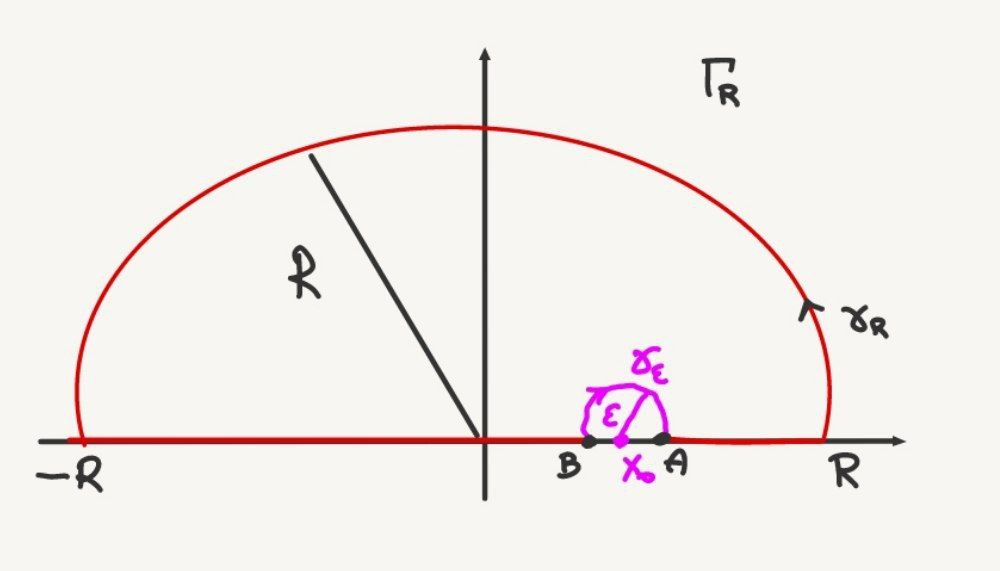
\includegraphics[width=0.5\linewidth]{immagini/fig1}
		\label{fig:fig1}
	\end{figure}

	\[I(R) = \int_{\Gamma_R} \frac{f(z)}{z-x_0}\,dz = 2\pi i \sum_k Res\Bigl[\frac{f(z)}{z-x_0},z_k\Bigr]\]
	Allora
	\begin{equation}
		P.V. \int_{-\infty}^{\infty} \frac{f(x)}{x-x_0}\,dx = \pi i f(x_0) + 2\pi i \sum_k Res\Bigl[\frac{f(z)}{z-x_0},z_k\Bigr]
	\end{equation}

\chapter{Proprietà mapping}

	Una funzione $f(z)$ può essere vista come una mappa da $\C \rightarrow \C$ \newline
	Dato un aperto $\Omega \subseteq D$ dominio di olomorfia, studio comportamento locale di $f$ per capire cosa succede a $f(\Omega) = \{f(z) \quad \vert \quad z \in \Omega\}$: \newline
	f è olomorfa $\Rightarrow$ f è analitica $\Rightarrow$ f è sviluppabile in serie di Taylor attorno a $z_0 \in \Omega$ \newline
	Il comportamento locale di f ha determinato dai primi termini della \hyperref[eq:taylor]{serie di taylor} \newline
	m è il primo indice tale che $a_m \neq 0$ $\Rightarrow$ il comportamento locale è determinato da 
	\[f(z)-f(z_0) \simeq a_m(z-z_0)^m\]
	Ci sono due casi:
	
	\begin{enumerate}
		\item $m=1$ \quad cioè \quad $a_1=f'(z_0)\neq0$
		
		\begin{teo}\hfil\\
			Esiste un aperto $U$ in un intorno di $z_0$ tale che:
			\begin{itemize}
				\item $f \text{ mappa } U$ in un intorno di $f(U)$ in maniera biunivoca
				\item $f(U)$ è un aperto $\Rightarrow$ f è una mappa aperta
				\item $f$ ha una funzione inversa $f^{-1}$ olomorfa e manda $f(U) \rightarrow U$
				\item $f$ è una mappa CONFORME, cioè converva gli ancoli tra le linee
			\end{itemize}
		\end{teo}
	
		\begin{Def}
			Dire che gli angoli si preservano significa che se le rette L e L' hanno angolo $\theta$ fra loro su U $\Rightarrow$ $f(L)$ e $f(L')$ hanno tangenti che si intersecano con angolo $\theta$ su $f(U)$ 
		\end{Def}
	
		$f$ manda rette in curve, ma le tangenti preservano gli angoli
		
		\begin{oss}
			Dato che $f^{-1}$ è olomorfa allora si può espandere in serie di Taylor attorno a $w_0=f(z_0)$
			\[f^{-1}(w) = \sum_{k=0}^{\infty} b_k (w-w_0)^k\]
			con i $b_k$ dati dalla formula di Lagrange
			\[b_0 = z_0 \qquad b_n = \frac{1}{n!} \frac{d^{n-1}}{dz^{n-1}} {\Bigl(\frac{z-z_0}{f(z)-f(z_0)}\Bigr)}^n \Bigr|_{z=z_0} \, n\geq 1\]
		\end{oss}
	
		\item $m>1$ si può dimostrare che esiste un aperto $U$ tale che 
		\begin{itemize}
			\item $f$ è una mappa m a 1 
			\item $f(U)$ è un aperto
			\item $f$ ingrandisce gli angoli di un fattore m
		\end{itemize}
	
	\end{enumerate}

	\begin{teo}[\textbf{Open Mapping}]\hfil\\
		Ogni funzione $f$ olomorfa non costante mappa aperti in aperti
	\end{teo}

	\begin{nb}
		Questo non vale se la funzione è costante perchè $f$ mappa $\C$ in un punto
	\end{nb}

	\begin{teo}\hfil\\
		Se $f$ è olomorfa e biunivoca si ha: 
		\[f'(z_0) \neq 0\ \; \forall z  \qquad \exists \, f^{-1} \text{ olomorfa }\]
		Si dice che $f$ è una MAPPA CONFORME
	\end{teo}

\section{Trasformazioni lineari fratte}
	Trasformazioni lineari conformi del tipo:
	\[F(z) = \frac{az + b}{cz + d} \qquad a,b,c,d \in \C\]
	con $ad-cb \neq 0$ sono mappe conformi $\forall z_0$ tali che $z_0 \neq -\frac{b}{c}$ \newline
	Inoltre
	\[F'(z) = \frac{ad-bc}{{cz+d}^2} \neq 0 \]
	Casi particolari:
	\begin{enumerate}
		\item Traslazioni: \qquad $w = z + \alpha$
		\item Dilatazioni: \qquad $w = \beta z$
		\item Inversioni:  \qquad $w = \frac{1}{z}$
	\end{enumerate}
	Qualsiasi $f$ lineare fratta può essere scitta come combinazione di queste 3 trasformazioni
	\begin{oss}
		Spesso conviene esprimere $F(z)$ sulla sfera di Riemann $\hat{\C} = \C \cup \{\infty\}$
		\[F\left(-\frac{d}{c}\right) = \infty \quad F(\infty) = \frac{a}{c} \qquad \text{quando } c=0 \to \infty\]
		Allora le trasformazioni lineari fratte sono le uniche mappe biunivoche e olomorfe di $\hat{\C} \rightarrow \hat{\C}$ \newline
		Sono AUTOMORFISMI  di $\hat{\C}$ \newline
		Mappano rette e cerchi in se stessi (in realtà su $\hat{\C}$ le rette sono cerchi che passano da $\infty$) \newline
		Inoltre dati 3 punti $z_1,z_2,z_3$ e dati $w_1,w_2,w_3$ esiste una sola trasformazione F che abbia 
		\[w_i = F(z_i) \; i=1,2,3\]	
	\end{oss}
	\begin{nb}
		\[B(z,z_1,z_2,z_3) = \frac{(z-z_1)(z_2-z_3)}{(z-z_3)(z_2-z_1)}\]
		è invariante sotto trasformazioni lineari fratte
		\[B(F(z),F(z_1),F(z_2),F(z_3)) = B (z,z_1,z_2,z_3)\]
	\end{nb}
	\begin{oss}
		L'insieme delle trasformazioni $F$ forma un gruppo. Associamo a $F$ la matrice 
		\[
		\hat{F} = 
		\left(\begin{matrix}
			a & b \\ c & d
		\end{matrix}\right)
		\qquad F = \frac{az + b}{cz+d}
		\]
		Inversa e composizione di $F$ seguono dalle regole delle matrici \newline
		Dato che si può riscalare $\hat{F} \rightarrow \lambda \hat{F}$ con $\lambda \in \C$ senza cambiare trasformazione allora si può normalizzare $\hat{F}$ in modo che $ ad-cb = 1$ \newline
		Quindi il gruppo delle trasformazioni $F$ è $SL(2, \C)$ gruppo di matrici $2 \times 2$ complesse e determinante unitario \newline
		Dato che $\det \hat{F} = 1$ non fissa il segno di $a,b,c,d$ ho che il gruppo è:
		\[\frac{Sl(2,\C)}{\mathbb{Z}_2} \qquad \mathbb{Z}_2 = \{\mathbb{I}, - \mathbb{I}\}\] 
	\end{oss}
	\begin{teo}[\textbf{Riemann mapping}]\hfill\\
		Ogni aperto semplicemente connesso $\omega \subset \C$ può essere mappato conformemente (cioè usando $f$ bi-olomorfa) sul cerchio unitario aperto
	\end{teo}
	\begin{coro}
		Tutte le regioni aperte di $\C$ semplicemente connesse sono uniformemente equivalenti 
	\end{coro}

\part{Spazi funzionali}

Vogliamo estendere la definizione di spazi euclidei $\R^3$ in maniera astratto in mdo da poterli usare anche per spazi$\infty-$dimensionali

\begin{Def}
	Uno \textbf{SPAZIO VETTORIALE V} su uno campo F è un insieme con 3 operazioni, chiuso rispetto:
	\begin{enumerate}
		\item somma per elementi dello spazio (vettori)
		\[\forall \, \vec{v},\vec{w} \in V \Rightarrow \vec{v}+\vec{w} \in V\]
		\item moltiplicazione per un elemento di F (scalari)
		\[\forall \lambda \in F \; \forall \, \vec{v}\in V \Rightarrow \lambda\vec{v} \in V\]
	\end{enumerate}
\end{Def}

\noindent La somma di vettori è associativa, commutativa, con elemento neutro $\vec{0}$ e inverso -$\vec{v}$; inoltre è distributiva sul prodotto con $\lambda \in F$ 
\[\lambda (\vec{v}+\vec{w}) = \lambda\vec{v}+\lambda\vec{w}\]
e ha elemento neutro prodotto $1\in F$

\begin{Def}
	$W \subset V$ è un \textbf{SOTTOSPAZIO} di V se è chiuso rispetto alla somma e moltiplicazione per uno scalare
	\begin{gather*}
		\forall\, \vec{v}, \vec{w} \in W \Rightarrow \vec{v}+\vec{w}\in W \subset v \\
		\forall \, \vec{v} \in W \; \forall \lambda \in F \Rightarrow \lambda \, \vec{v} \in W \subset V 
	\end{gather*}
\end{Def}

\begin{Def}
	n vettori $\vec{u}_k \; k = 1, \dots , n$ sono \textbf{lineramente indipendenti} se 
	\[\sum_{k=1}^n a_k \vec{u}_k = 0 \Rightarrow \forall k = 1,\dots,n 	\; a_k=0\]
\end{Def}

\begin{Def}
	Invece sono \textbf{lineramente dipendenti} se 
	\[\sum_{k=1}^n a_k\vec{u}_k = 0 \qquad \text{con qualche } a_k \ne 0\]
\end{Def}

\begin{Def}
	Un insieme di vettori linearmente indipendenti è detto \textbf{massimale} se l'insieme dei vettori linearmente indipendeti + uno qualsiasi altro vettore è linearmente dipendente \newline
	\{$u_k$\} è chiamata \textbf{base} di V
\end{Def}

\begin{oss}
	Data una base posso scrivere un qualsiasi vettore $\vec{v}\in V$ in coordinate o componenti
	\[\vec{v} = \sum_{k=1}^n v_k\vec{u}_k \qquad v_k \in F\]
\end{oss}

\begin{oss}
	n può essere finito o infinito; se è finito tutte le basi hanno lo stesso numero di vettori e si chiama \textbf{dimensione} dello spazio \newline
	Gli spazi di funzioni sono un esempio di spazio $\infty-$dimensionali
\end{oss}

\noindent Sugli spazi vettoriali astratti è possibile aggiungere strutture che permettorno di specificare il concetto di lunghezza o distanza, il concetto di limite e di continuità in maniera astratta

\begin{Def}
	Una \textbf{metrica o distanza} è una mappa 
	\[d(,): \, M \to \R\]
	con le seguenti proprietà valide $\forall a,b \in M$
	\begin{gather*}
		d(a,b) = d(b,a) \\
		d(a,b) = 0 \iff a=b \\
		\forall c \in M \quad d(a,b)+d(b,c) \ge d(a,c)
	\end{gather*}
\end{Def}

\begin{Def}
	Uno spazio vettoriale i cui è possibile definire una matrica è uno \textbf{spazio metrico}
\end{Def}

\begin{Def}
	Una \textbf{topologia} su un insieme X è una collezione $\tau$ di sottoinsiemi di X che contiene l'insieme vuoto, X stesso e che deve essere chiusa rispetto ad un numero finito di iterazioni e ad un numero arbitrario di interazioni, cioè
	\begin{itemize}
		\item $\emptyset \in \tau$
 		\item $X in \tau$
		\item $\forall \, V_i \in Z \quad V_1 \cap V_2 \cap \dots \cap V_n \in \tau $
		\item $\cup_\alpha \quad V_\alpha \in \tau$ \; con $\alpha$ finito o infinito
	\end{itemize} 
	Gli elementi di $\tau$ sono gli insiemi aperti 
\end{Def}

\begin{oss}
	La topologia non è unica
\end{oss}

\begin{Def}
	Una \textbf{sfera aperta} di raggio r centrata in $a \in M$ è
	\[B(a,r) = \{b \in M \; | \; d(a,b)<r\}\]
\end{Def}

\begin{Def}
	Ogni sottoinsieme di $X\subset M$ è aperto se 
	\[\forall \, a_o \in X \quad \exists \, B(a_o,r) \subset X\]
\end{Def}

\begin{oss}
	Ogni spazio metrico è uno spazio topologico, basta definire la topologia degli aperti tramite sfere aperte
\end{oss}

\begin{Def}
	Un insieme è \textbf{chiuso} se il suo complementare è aperto
\end{Def}

\begin{oss}
	L'esistenza di una topologia metrica permette di definire la nozione di limite di una successione \;
	Diciamo che \{$a_n$\} converge ad $a\in M$ se 
	\[\forall \varepsilon>0 \quad \exists \, n_o \text{ tale che } d(a_n, a)<\varepsilon \quad \forall \, n>n_o\]
	oppure usando la definizione di limite di $\R$
	\[\lim_{n\to \infty} d(a_n,a) =0\]
\end{oss}

\begin{oss}
	La convergenza di una serie si prova con la convergenza delle somme parziali
\end{oss}

\begin{oss}
	Un insieme chiuso contiene tutti i suoi punti di accumulazione ed il più piccolo insieme chiuso che contiene X è detto \textbf{chiusura} di X ($\bar{X}$)
\end{oss}

\begin{Def}
	Un insieme Z si dice \textbf{denso} in Y se la sua chiusura corrisponde a $Y = \bar{Z}$
\end{Def}

\begin{Def}
	Un insieme K in uno spazio metrico X è \textbf{compatto} $\iff$ ogni succesione \{$X_k$\} interamente contenuta in K ha una sottosuccesione convergente ad un elemento di K
\end{Def}

\begin{Def}
	Una mappa
	\[f: \; X\to Y\]
	tra due spazi topologici è \textbf{continua} se la controimmagine di ogni aperto in Y contenente f($X_0$) è un aperto in X contenente $X_0$ \newline
	Per spazi metri è possibile formulare ciò con sfere aperte
	\[\forall\varepsilon> 0 \quad \forall \delta> 0 \text{ tale che } d(f(x),f(x_0))<\varepsilon \qquad \text{ se } d(x,x_0)<\delta\]
\end{Def}

\begin{Def}
	Una \textbf{successione di Cauchy} è una succesione \{$x_n$\} tale che 
	\[\forall \varepsilon>0 \quad \exists \; N_\varepsilon >0 \text{ tale che } \forall \; n,m \ge N_\varepsilon \qquad d(x_n,x_m)< \varepsilon\]
\end{Def}

\begin{teo}
	In uno spazio metrico ogni successione convergente è una successione di Cauchy 
\end{teo}

\begin{Def}
	Uno spazio metrico si dice \textbf{completo} se tutte le successioni di Cauchy sono convergenti 
\end{Def}

\chapter{Spazi normati}

\begin{Def}
	La \textbf{norma} di un vettore $\in V$ spazio vettoriale è una mappa
	\[||\,||: \; V \to \R^+\]
	che soddisfa $\forall \; \vec{v},\vec{w}\in V \quad \forall\lambda \in \C,\R$
	\begin{enumerate}
		\item $||\vec{v}||\ge 0 \qquad ||{\vec{v}}||=0 \iff \; \vec{v} = \vec{0}$ \qquad condizione di positività
	  	\item $||\lambda\vec{v}|| = \abs{\lambda}||\vec{v}||$
    \item $||\vec{v}+\vec{w}|| \le ||\vec{v}|| + ||\vec{w}||$ \qquad disuguaglianza triangolare
	\end{enumerate}
\end{Def}

\begin{Def}
	Uno spazio vettoriale dotato di norma si dice \textbf{spazio normato}
\end{Def}

\begin{coro}
	Gli spazi normati sono sempre degli spazi metrci dato che si può sempre definire
	\[d(\vec{v},\vec{w})= ||\vec{v}-\vec{w}||\]
\end{coro}

\begin{coro}
	Per la convergenza in uno spazio normato si può usare 
	\[\lim_{n\to\infty} ||\vec{v}_n - \vec{v}|| =0\]
\end{coro}

\begin{Def}
	Un \textbf{isomorfismo} tra spazi normati è una mappa biunivoca
	\[f: \; (X, ||\,||_x) \to (Y, ||\, ||_y)\]
	che preserva la struttura lineare e la norma, cioè
	\begin{itemize}
		\item $f(\lambda\vec{v}+\mu\vec{w}) = \lambda f(\vec{v})+ \mu f(\vec{w})$ 
  \item $||f(\vec{v})||_y = ||\vec{v}||_x \qquad \forall \;\vec{v},\vec{w} \in X \quad \lambda,\mu \in F$
	\end{itemize}
\end{Def}

\begin{oss}
	Tramite la norma superiore 
	\[||f||_{sup} = \sup_{x\in K} \abs{f(x)}\]
	possiamo definire il concetto di convergenza uniforme
\end{oss}

\begin{Def}
	$\{f_n\} \to f$ converge uniformemente su K se 
	\[\lim_{n\to\infty} \underbrace{\sup_{x\in K} \abs{f_n(x)-f(x)}}_{||f_n-f||_{sup}} =0\]
\end{Def}

\begin{oss}
	La convergenza uniforme inplica la convergenza puntuale
\end{oss}

\begin{Def}
	Norma $L_1$
	\[||f||_1 = \int_0^1 \abs{f(x)}\, dx\]
\end{Def}

\begin{oss}
	Si può dimostrare che la convergenza in norma sup implica convergenza in norma $L_1$
\end{oss}

\begin{Def}
	Uno \textbf{spazio di Banach} è uno spazio vettoriale normato e completo
\end{Def}

\begin{Def}
	Il \textbf{prodotto scalare (o interno)} su uno spazio vettoriale complesso è una mappa 
	\begin{align*}
		(\vec{a},\vec{b}): \; V\times V &\to \C \\
		\vec{v},\vec{w} &\mapsto (\vec{v},\vec{w})
	\end{align*}
	che soddisfa le seguenti proprietà:
	\begin{enumerate}
		\item Linearità
		\[(\vec{u}, \lambda\vec{v}+\mu\vec{w}) = \lambda(\vec{u}, \vec{v}) + \mu(\vec{v},\vec{w}) \qquad \forall\lambda,\mu \in \C\]
		\item Hermiticità \label{2}
		\[(\vec{v}, \vec{w}) = \overline{(\vec{w},\vec{v})} \quad \text{ simmetria su $\R$}\]
		\item Positività
		\[(\vec{v},\vec{v})\ge 0 \qquad (\vec{v},\vec{v})=0 \iff \vec{v} = \vec{0}\]
	\end{enumerate}
\end{Def}

\begin{oss}
	La prop \hyperref[2]{2} implica anti-linearità nel primo argomento
	\[(\lambda\vec{u}+\mu\vec{v}, \vec{w}) = \bar{\lambda}(\vec{u},\vec{w})+\bar{\mu}(\vec{v},\vec{w})\]
\end{oss}

\begin{Def}
	Uno spazio vettoriale dotato di prodotto scalare è detto \textbf{pre-Hilbert}
\end{Def}

\begin{oss}
	Pre-Hilbert è anche uno spazio normato; si può sempre definire
	\[||\vec{v}|| = \sqrt[]{(\vec{v}, \vec{v})}\]
\end{oss}

\begin{oss}
	Il prodotto scalare soddisfa la disuguaglianza di Schwarz
	\[{\abs{(\vec{v},\vec{w})}}^2 \le (\vec{v},\vec{v})(\vec{w},\vec{w})\]
\end{oss}

\begin{Def}
	Uno \textbf{spazio di Hilbert finito dimensionale} è uno spazio vettoriale dotato di prodotto scalare e completo 
\end{Def}

\begin{Def}
	Due vettori sono \textbf{ortogonali} se il loro prodotto scalare è nullo
	\[(\vec{v},\vec{w})=0\]
\end{Def}

\begin{oss}
	I vettori ortogonali sono linearmente indipendenti 
\end{oss}

\begin{oss}
	Gli elementi di una base (set massimale di vettori linearmenti indipendenti) sono \textbf{ortomormali}
	\[(\vec{e}_i,\vec{e}_j) = \delta_{ij} \quad \forall \; i,j = 1,\dots,n\]
	\begin{enumerate}
		\item $\vec{v} = \displaystyle \sum_{k=1}^n v_k \vec{e}_k \qquad v_k = (\vec{e}_k,\vec{v})$
  \item $(\vec{v},\vec{w})= \displaystyle \sum_{k=1}^n \bar{v}_k\vec{w}_k \qquad \bar{v}_k = (\vec{v}, \vec{e}_k) \quad \vec{w}_k = (\vec{e}_k,\vec{w})$
  \item ${||\vec{v}||}^2 = \displaystyle \sum_{k=1}^n {\abs{v_k}}^2$ identità di Parseval
	\end{enumerate}
\end{oss}

\begin{oss}
	In ogni spazio di Hilbert finito dimensionale è sempre possibile costruire una base ortonormale a partire da qualsiasi base 
\end{oss}

\chapter{Spazi di Hilbert infinito dimensionali}
Ci concentriamo sugli spazi separabili, cioè che hanno un sottoinsieme denso che è contabile \newline
Diciamoc che il set $\{\vec{l}_k\}$ con $k\in \mathbb{N}$ in uno spazio di Hilbert infinito dimensionale è un sistema ortonormale Se
\[(\vec{e}_i,\vec{e}_j) = \delta_{ij} \quad \forall \, i,j \in \mathbb{N} \]
Se inoltre $\forall \vec{v}$ si può scrivere
\[\vec{v} = \sum_[i=1]^\infty v_i\vec{e}_i \qquad v_i = (\vec{e}_i,\vec{v})\in \C\]
allora il sistema $\{\vec{e}_k\}$ è un \textbf{sistema ortonormale completo} [S.O.N.C] o base di Hilbert

\begin{oss}
	Abbiamo generalizzato la nozione di base usando $\infty$ elementi; ciò è possibile perchè abbiamo la nozione di limite
	\[\vec{v} = \lim_{n\to\infty} \sum_{i=1}^n v_i\vec{e}_i \qquad \vec{v} = \lim_{n\to\infty} \left|\left| \sum_{i=1}^n v_i\vec{e}_i - \vec{v}\right| \right| =0\] 
\end{oss}

\begin{Def}
	L'espansione 
	\[\vec{v} = \sum_{i=1}^\infty (\vec{e}_i,\vec{v})\vec{e}_i\]
	è chiamata \textbf{serie di Fourier} e i coefficienti $v_i$ sono detti coefficienti di Fourier
\end{Def}

\begin{teo}
	La serie $\displaystyle \sum_{i=1}^n \alpha_i\vec{e}_i$ converge $\iff \displaystyle \sum_{i=1}^\infty {\abs{\alpha_i}}^2$ converge 
\end{teo}

\begin{oss}
	Come nel caso finito dimensionale valgono
	\begin{itemize}
		\item $(\vec{v},\vec{e}_i) = 0 \quad \forall i \Rightarrow \vec{v}=0$
  \item $||\vec{v}|| = \displaystyle \sum_{k=1}^\infty {\abs{v_k}}^2 \quad \forall\vec{v}$
  \item $\forall \; \vec{v},\vec{w} \in V \Rightarrow (\vec{v},\vec{w}) = \displaystyle \sum_{k=1}^\infty \bar{v}_kw_k$
	\end{itemize}
\end{oss}

\begin{Def}
	Lo spazio $l^2(\C)$
	\[\sum_{n=1}^\infty {\abs{z_n}}^2 < \infty\]
	è uno spazio di Hilbert con il prodotto scalare \newline
	In generale gli spazi $l^p(\R)$ o $l^p(\C)$ con $1 \le p <\infty$
	\[\sum_{n=0}^\infty {\abs{x_n}}^p < \infty\]
	sono solamente dotati di norma, quindi sono spazi di Banach 
\end{Def}

\begin{oss}
	Si può dimostrare utilizzando la disuguaglianza di Minkowski per le serie 
	\[{\left(\sum_{n=0}^\infty {\abs{x_n+y_N}}^p\right)}^{\frac{1}{p}} \le {\left(\sum_{n=0}^\infty {\abs{x_n}}^p\right)}^{\frac{1}{p}} + {\left(\sum_{n=0}^\infty {\abs{y_n}}^p\right)}^{\frac{1}{p}}\]
\end{oss}

\begin{Def}
	Gli spazi $l^\infty(\R/\C)$ sono anch'essi spazi di Banach formati da successioni limitate e dotati di norma superiore
	\[\sup_{0\le n \le \infty} \abs{x_n} < \infty\]
\end{Def}

\noindent Il tipico esempio di prodotto scalare su spazi di Hilbert infinito dimensionale è quello di funzioni sull'intervallo $[a,b]$
\[(f,g) = \int_a^b \bar{f}(x)g(x) \, dx\]
La somma $L^1$ rientra in questa categoria

\section{Integrali}
\subsection*{Integrale di Riemann}
\[I = \sum_{i=1}^n (x_{i+1}-x_i)f(\bar{x}_i)\]
Quando esiste finito il limite per $n \to \infty \; x_{i+1}-x_i \to \infty$ si dice INTEGRALE DI RIEMANN  e la funzione si dice integrabile secondo Riemann 

\subsection*{Integrale Lebesgue}
\[I = \sum_{i=1}^n f_i\mu (f^{-1}([f_{i+1}-f_i]))\]
con $f_i$ una partizione del range di f e con $\mu(x)$ misura di X \newline
La controimmagine di un intervallo non è necessariamente un intervallo 

\chapter{Spazio \texorpdfstring{$L^1_w (\Omega)$}{U}}
\begin{Def}
	Lo spazio $L^1_w(\Omega)$ è uno spazio di funzioni definite su un insieme $\Omega\subset \R/\C$, Lebesgue-integrabili con norma
	\[||f||_1 = \int_\Omega \abs{f(x)}\underbrace{w(x)}_{misura} \, dx <\infty\]
\end{Def}

\noindent Questi spazi $L^1_w(\Omega)$ sono spazi di Banach 

\begin{oss}
	Lo spazio delle funzioni continue su un intervallo $C([a,b])$ con norma 
	\[L^1 = \int_a^b f(x) \, dx \]
	non è uno spazio di Banach, perchè non è completo 
\end{oss}

\begin{oss}
	Se vogliamo che lo spazio $L^1_w(\Omega)$ sia uno spazio di Banach dobbiamo provare linearità, positività e disuguaglianza triangolare nella norma $L^1_w$ \newline
	La linearità e la disuguaglianza trinagolare seguono facilmente dalle proprietà degli integrali, la positività vera per integrale di Riemann, ma non è più vera in generale per integrale di Lebesgue; dobbiamo allora definire $f(x)=0$ quasi ovunque
\end{oss}

\begin{teo}[Riesz-Fischer] \label{teo:riesz}
	$L^1_w$ è completo e quindi di Banach 	
\end{teo}

\begin{nb}
	Per dimostrare che questo spazio è completo, bisogna usare ben due teoremi dell'integrale di Lebesgue $\Rightarrow$ questo vale solo per funzioni Lebesgue-integrabili 
\end{nb}

\section{Spazi \texorpdfstring{$L^p_w(\Omega)$}{U}}
Spazio delle funzioni a valori complessi du regione $\Omega \subset \R^n/\C^n$ tale che 
\[\int_\Omega {\abs{f(x)}}^p w(x)\, dx < \infty \qquad p \ge 1 \in \R \]

\begin{oss}
	Le funzioni uguali quasi ovunque sono considerate identiche
\end{oss}

\begin{oss}
	Gli spazi $L^p_w(\Omega)$ sono spazi di Banach con norma $L^p_w$
	\[||f||_p = {\left(\int_\Omega {\abs{f(x)}}^p w(x) \, dx \right)}^{\frac{1}{p}}\]
	La completezza di questi spazi si può dimostrare generalizzando il \hyperref[teo:riesz]{teorema di Riesz-Fischer}
\end{oss}

\begin{oss}
	Ci sono due ulteriori disuguaglianze notevoli; se assumiamo che p e q siano coniugati, cioè $\frac{1}{p} + \frac{1}{q} = 1$ allora valgono
	\begin{enumerate}
		\item Disuguaglianza di Holder
		\[||fg||_p \le ||f||_p ||g||_p\]
		\item Disuguaglianza di Minkowski
		\[||f+g||_p \le ||f||_p + ||g||_p\]
	\end{enumerate}
\end{oss}

\begin{oss}
	Tra tutti i p possibili, il caso p=2 è particolare; $L^2_w(\Omega)$ non è solo uno spazio di Banach, ma anche uno spazio di Hilbert. E\' infatti l'unico su cui si può definire il prodotto scalare 
	\[(f,g) = \int_\Omega \bar{f}(x)g(x)w(x) \, dx \]
	che induce norma $L^2_w$
	\[||f||_2 = {((f,f))}^{\frac{1}{2}} = {\left(\int_\Omega {\abs{f(x)}}^2 w(x) \, dx\right)}^{\frac{1}{2}}\]
	$L^2_w(\Omega)$ è lo spazio delle funzioni a quadrato integrabile e contiene sia funzioni continue $C(\Omega)$ sia funzioni con singolarità  
\end{oss}

\chapter{Basi di Hilbert ed espansione di Fourier}

Applicando la teoria generale degli spazi di Hilbert a $L^2_w(\Omega)$ si arriva alla conclusione che è possibile definire una base contabile di funzioni in $L^2_w(\Omega)$ \newline
Quindi una qualsiasi funzione $f\in L^2_w(\Omega)$ può essere espressa come combinazione degli infiniti elementi della base ortogonale

\section{Basi ortonormali}

Una funzione si dice normalizzata se la sua norma è 1; in particolare per $L^2_w(\Omega)$

\begin{equation*}
	\label{eq:1.1}
	{||f||}_2 = \int_\Omega \abs{f(x)}^2w(x) \, dx = 1
\end{equation*}

\begin{Def}
	\label{def:ortogonali}
	Due funzioni sono \textbf{ortogonali} se 
	\begin{equation*}
		(f,g) = \int_\Omega \overline{f(x)}g(x)w(x) \, dx = 0
	\end{equation*}
\end{Def}

\begin{Def}
	\label{def: base ortonormale}
	Una \textbf{base ortonormale} è un set di funzioni $\Psi_n(x)$ con $n = 0,1,\dots,N$ su $L^2_w(\Omega)$ che soddisfano
	\begin{equation*}
		(\Psi_n,\Psi_m) = \delta_{m,n} \qquad \forall \; m,n = 0,1,\dots,N 
	\end{equation*}
\end{Def}

\begin{oss}
	Se non ci sono altre funzioni ortogonali a tutti $\Psi_n$ allora il sistema è completo. Quindi \{$\Psi_n$\} è una base di Hilbert di $L^2_w(\Omega)$
\end{oss}

\noindent Per la teoria generale degli spazi di Hilbert si può perciò espandere qualsiasi funzione $f\in L^2_w(\Omega)$ sulla base 
\begin{equation*}
	\sum_{n=0}^\infty C_n \Psi_n \qquad \text{serie di Fourier}
\end{equation*}
I coefficienti di Fourier $C_n$ si calcolano
\begin{equation*}
	C_n = (\Psi_n,f) = \int_\Omega \overline{\Psi_n(x)}f(x)w(x) \, dx 
\end{equation*}

\begin{oss}
	La convergenza della serie di Fourier non implica che 
	\begin{equation*}
		\sum_{n=0}^\infty C_n\Psi_n
	\end{equation*}
	converga puntualmente (cioè $\forall \, x$) ad f, ma va intesa come convergenza in norma $L^2_w(\Omega)$, cioè
	\begin{equation*}
		\lim_{n\to\infty} \int_\Omega {\abs{f(x) - \sum_{n=0}^n C_n\Psi_n}}^2 w(x) \, dx =0
	\end{equation*}
\end{oss}

\begin{oss}
	La serie di Fourier di una qualsiasi funzione a quadrato integrabile definita su $[a,b]$ converge alla funzione stessa in norma $L_2$
	\begin{equation*}
		\lim_{n\to\infty} {||\sum{k=-n}^n c_k \Psi_k - f||}_2 =0
	\end{equation*}
\end{oss}

\begin{oss}
	Se $f(x)\in\R \Rightarrow c_k = \overline{c}_{-k}$
\end{oss}

\begin{oss}
	La serie di Fourier su $L^2_{[a,b]}$ può essere anche scritta in forma trigonometrica usando 
	\begin{equation*}
		e^{\pm 2\pi in \frac{x}{L}} = \cos{\left(\frac{2\pi nx}{L}\right)} \pm i\sin{\left(\frac{2\pi nx}{L}\right)}
	\end{equation*}
	per cui 
	\begin{equation*}
		f(x) = \frac{a_0}{2} + \sum_{n=1}^\infty a_n \cos{\left(\frac{2\pi nx}{L}\right)} + \sum_{n=1}^\infty \sin{\left(\frac{2\pi nx}{L}\right)}
	\end{equation*}
	In questa formulazione i coefficienti sono dati da 
	\begin{gather*}
		a_n = \frac{c_n + c_{-n}}{\sqrt[]{2}} \qquad b_n = \frac{i(c_n - c_{-n})}{\sqrt[]{2}} \\
		a_n = \frac{2}{L} \int_a^b f(x) \cos{\left(\frac{2\pi nx}{L}\right)} \, dx \qquad  b_n = \frac{2}{L} \int_a^b f(x) \sin{\left(\frac{2\pi nx}{L}\right)} \, dx 
	\end{gather*}
	Quindi la base della forma trigonometrica è data da 
	\begin{equation*}
		\left\{\frac{1}{\sqrt[]{L}}, \sqrt[]{\frac{2}{L}} \cos{\left(\frac{2\pi nx}{L}\right)}, \sqrt[]{\frac{2}{L}} \sin{\left(\frac{2\pi nx}{L}\right)}\right\} \qquad n>1
	\end{equation*}
	Le funzioni della base trigonometrica si chiamano \textbf{armoniche} e il numero $\frac{n}{L}$ si dice frequenza dell'armonica
\end{oss}

\begin{oss}
	Per definire i coefficienti della serie di Fourier 
	\begin{equation*}
		c_n = \frac{1}{\sqrt[]{L}} \int_a^b e^{-2\pi i \frac{nx}{L}} f(x) \, dx
	\end{equation*}
	basta che $f(x)\in L^1_{[a,b]}$ e non per forza in $L^2_{[a,b]}$
\end{oss}

\section{Convergenza puntuale}

Per semplicità assumiamo $[a,b] = [0,2\pi]$ \newline
Se prendo $f(x)\in L^1_{[0,2\pi]}$ allora 
\begin{equation*}
	c_n =(\Psi_n,f) = \frac{1}{\sqrt[]{2\pi}}\int_0^{2\pi} e^{-inx} f(x)
\end{equation*}
sono ben definiti e si può costruire la serie di Fourier
\begin{equation*}
	\frac{1}{\sqrt[]{2\pi}} \sum_{n=-\infty}^\infty c_n e^{inx}
\end{equation*}
Osservo che la serie di Fourier ha termini che sono periodici con periodo $2\pi$
\begin{equation*}
	e^{inx} = e^{i(nx+2\pi)}
\end{equation*}
Quindi posso estendere le funzioni f da $[0,2\pi]$ a tutto $\R$ usando le condizioni periodiche per l'estensione
\begin{equation*}
	f(x+2\pi) = f(x)
\end{equation*}
Allora posso studiare su tutto $\R$ la convergenza delle somme parziali
\begin{equation*}
	S_n(x) = \frac{1}{\sqrt[]{2\pi}} \sum_{k=-n}^n c_ke^{-ikx} = \sum_{k=-n}^n \frac{1}{2\pi} \left[\int_0^{2\pi} e^{-iky}f(y) \, dy\right] e^{-ikx} = \frac{1}{2\pi}\int_0^{2\pi} \sum_{k=-n}^n e^{ik(x-y)}f(y) \, dy 
\end{equation*}
ora sfrutto la periodicità di f per cambiare variabile $z = x-y$ dato che 
\begin{equation*}
	\int_{a+2\pi}^{b+2\pi} f(x)\, dx = \int_a^b f(x) \, dx 
\end{equation*}
Allora ottengo
\begin{equation*}
	S_n(x) = \frac{1}{2\pi} \int_0^{2\pi} \sum_{k=-n}^n e^{ikz}f(x+z) \, dz
\end{equation*}
introduco KERNEL DI DIRICHLET
\begin{equation*}
	D_n(z) = \sum_{k=-n}^n e^{ikz} = \frac{\sin{\left(\frac{2n+1}{2}z\right)}}{\sin{\left(\frac{z}{2}\right)}}
\end{equation*}
per riscrivere
\begin{equation*}
	S_n = \frac{1}{2\pi} \int_0^{2\pi} f(x+z)D_n(z) \, dz
\end{equation*}
dividendo integrale ottengo
\begin{equation*}
	S_n(x) = \frac{1}{\pi} \int_0^\pi \frac{f(x+z)-f(x-z)}{2}D_n(z)
\end{equation*}

\begin{teo}[Dirichlet]\hfill\\
	Data f con periodo $2\pi$  che sia $L^1_{[0,2\pi]}$ tale che 
	\begin{equation*}
		\lim{y\to x^{\pm}} f(y) = f(x^{\pm})	
	\end{equation*}
	e tale che esista integrale 
	\begin{equation*}
		\int_0^\delta \frac{f(x\pm y)-f(x^{\pm})}{y} \, dy
	\end{equation*}	
	per qualche valore di $\delta$, allora la serie di Fourier 
	\begin{equation*}
		\frac{1}{\sqrt[]{2\pi}} \sum_{n=-\infty}^\infty c_n e^{inx}
	\end{equation*}
	converge a 
	\begin{equation*}
		\begin{cases}
			f(x) \qquad &\text{se f è continua}\\
			\frac{1}{2}[f(x^+)+f(x^-)] \qquad & \text{se f è discontinua}
		\end{cases}
	\end{equation*}
\end{teo}

\begin{oss}
	Il teorema di Dirichlet si applica a tutte le funzioni $C^1$ a pezzi 
\end{oss}

\section{Polinomi ortonormali}



\end{document}